\section{The building blocks: basic algorithms}
The following section defines the basic methods upon which the contribution builds. It begins by describing a weighted particle filter for probabilistic state-estimation, a Monte Carlo Search Tree, and finally describes the architecture of a (modified) Multi-Agent Partially Observable Monte Carlo Planner \cite{Hayashi_et_al2020,Silver2010}.  
\subsection{Particle Filtering: iterative approximate Bayesian Updates}\label{ParticleFiter}
Traditionally the use of Bayes Law is used iteratively in each timestep to reason over uncertain information to update the posterior probability of being in a certain state.
\begin{equation}
    b_{t+1}(s') = \frac{O^{s' a_t z_{t+1}} \Sigma_{s \in S} P^{s a_t s'} b_t (s)}{\Sigma_{s'' \in S} O^{s'' a_t z_{t+1}}  \Sigma_{s \in S} P^{s a_t s''} b_t (s)}
\end{equation} 
% This shows the computation necessary: the belief update over the state is equal to the probability of recieving an observation in state $s'$ given the previous action and observation. This is multiplied by summing over the transition probabilities of taking an action in the previous state, given the previous belief state. Finally this is all normalised over the sum over all possible states of the observation of reciving this observation, given the previous state and action if not in state $s'$ multiplies by the sum over the transition probabilies of moving from the previous state having taken action $a_t$ and arriving in not state $s'$ multiplied by the previous beliefs.
\newline \newline
In complex environments (particularly those where there are multiple opponents), performing a complete Bayesian update can be so costly as to be intractable. Hence, recent works in opponent modelling have used deep-learning to approximate the update (see for example \cite{he_om_DRL}). However deep-neural nets require training, and can take many iterations before being successful. A recent strategy for opponent modelling (adapted by \cite{Hayashi_et_al2020}), however proposed to expand Monte-Carlo planning to partially observable domains is a sampling based approach which makes use of a generative environment model. This environment model ($G$) can be used to perform Bayesian Filtering. 
\newline \newline
The belief state (i.e. the belief distribution over possible states) is sampled for a history $h_t$ by $K$ particles, with index $i$ and a weighting of $w$ 
\begin{equation}
    k \in K, k = \langle i, w \rangle; B^i_t \in S, 1 < i < K    
\end{equation}
Each sample represents a possible state, and the belief-state is the weighted sum over all particles. 
\newline \newline
Particles are iteratively removed and reinvigorated at each timestep. At the start of a game/iteration, K particles are sampled from the initial belief-state. The agent selections an action $a_{t, real} \in A$, and receives an observation $o_{t+1,real}$. 
\newline \newline
Each particle is then evaluated. From the state in $K$, an agent uses the internal generative model to provide a sample of a successor observation: 
\begin{equation}
    o_{t+1, possible} = G(k_i, a_t)
\end{equation}
This possible state is then compared to the real observation via a distance metric to return a value of the accuracy of this particle $V(k)$, which in turn is used to update the value of each particles weighting ($w_k$) (by a learning rate denoted $\gamma$) 
\begin{equation}
    V(k_i) = o_{t+1, possible} - o_{t+1, real}
\end{equation}
\begin{equation}
    w_{k_i} \leftarrow w_k + (- \gamma * V(k_i))
\end{equation}
The weaker particles are pruned based on a hyperparameter depending on the relative strength of weightings. Finally, new particles are created by sampling and adding Gaussian noise to existing particles. 
\newline \newline
The result is that as the history increases (i.e. more observations are evaluated) the belief-state should converge as inaccurate state hypotheses are filtered, and more accurate hypotheses increasingly suggested. 

\subsection{Monte Carlo Tree Search --- an approach to search in a large state-space}\label{MCTSDesc}
Monte Carlo Tree Search is a sample-based search algorithm. 
Similar to a particle filter, it requires a generative model of the environment ($G$) to evaluate possible actions and future states in order to converge to an optimal policy online (i.e. re-evaluating from each state). 
\newline \newline
An agent begins in a state ($s_0 \in S$). From this state, it constructs a sample-based search tree of possible successor states.
\begin{equation}
    T \sim \langle N, E \rangle
\end{equation} 
\begin{equation}
    N \sim \langle s, q, v \rangle 
\end{equation}

In this search tree, each node ($n \in N$) represents a possible state ($s \in S$), and transitions (edges ($e \in E$) are possible (probabilistic) actions, mapping a node to a probable successor node given a state and action pair. 
\newline \newline
In each iteration, the tree is traversed in a best-first search procedure. Typically, the value of selecting a node is estimated by the upper-confidence trees algorithm (an adapted upper confidence bound UCB1 bandit algorithm). This weights the relative value of the explored node with an exploration value (derived by the expression on the far right of equation \ref{UCB1}) which weights the number of times that node has been explored relative to its parent node, by the scalar constant $c$ (which typically takes the value of 2).
\begin{equation}\label{UCB1}
    V(n \in N) = V(n) + c \sqrt{\frac{log(parent(n)_{visits})}{n_{visits}}} 
\end{equation}
Given a sufficiently large tree, this approach has shown to converge (eventually) to an optimal policy \cite{Ross2011}. 
Having reached a leaf node (i.e. a node in the tree $T$ with no children), children are generated by \textit{expanding} the node. In this case, all possible successor states of the node are created and added to the tree by use of the generative environment model $G$. 
\begin{equation}
    s_{t+1, possible} \leftarrow G(s_t, a_t)
\end{equation}
Having generated the successor states, the agent estimates the value of each state by performing random \textit{rollouts} to a predetermined depth. These \textit{simulations} (sometimes referred to as \textit{rollouts}) take the form of a random sequence of actions, and return the rewards for the successive states. The reward of potential future states are sampled from these rollouts by taking the mean eventual reward for a single starting state. For $x$ number of rollouts:
\begin{equation}
    Q(n \in N) = \frac{1}{x}\Sigma_{i=0}^x R^i
\end{equation} 
where $R^i$ is the reward over the $i^{th}$ rollout.
\newline\newline
Finally, the estimated values of the leaf nodes are backpropagated throughout the tree, in order to allow for potential future states to add value to their parent states, until finally all the possible moves available in the initial state (the root node) have accurate values, from which one can select an optimal action. 
\newline \newline
For a fixed time-period or for a fixed number of simulations, the cycle of \textit{tree-traversal}: traversing the tree $T$; \textit{expansion}: simulating all possible actions in a given state to add all possible successor states to the tree; \textit{Simulation/rollouts}: performing random rollouts to estimate the value of the state; and \textit{backpropagation}: propagating expected rewards back up the tree. This cycle then continues for a determined period, until a new action is selected, and a new state observed. 
\newline \newline
This approach, typically when paired with a strong heuristic and an accurate transition/environment simulator, has shown to be an effective and powerful approach to action-selection in complex environments with large search spaces --- this algorithm forms the basis for most of the recent successes in adversarial AI (as described in more detail in Section \ref{RL + Search}) 

\begin{figure*}
    \caption{Graphical representation of the four stages of a single iteration a Monte Carlo Tree Search, where $X$ represents the number of samples taken per timestep.}
    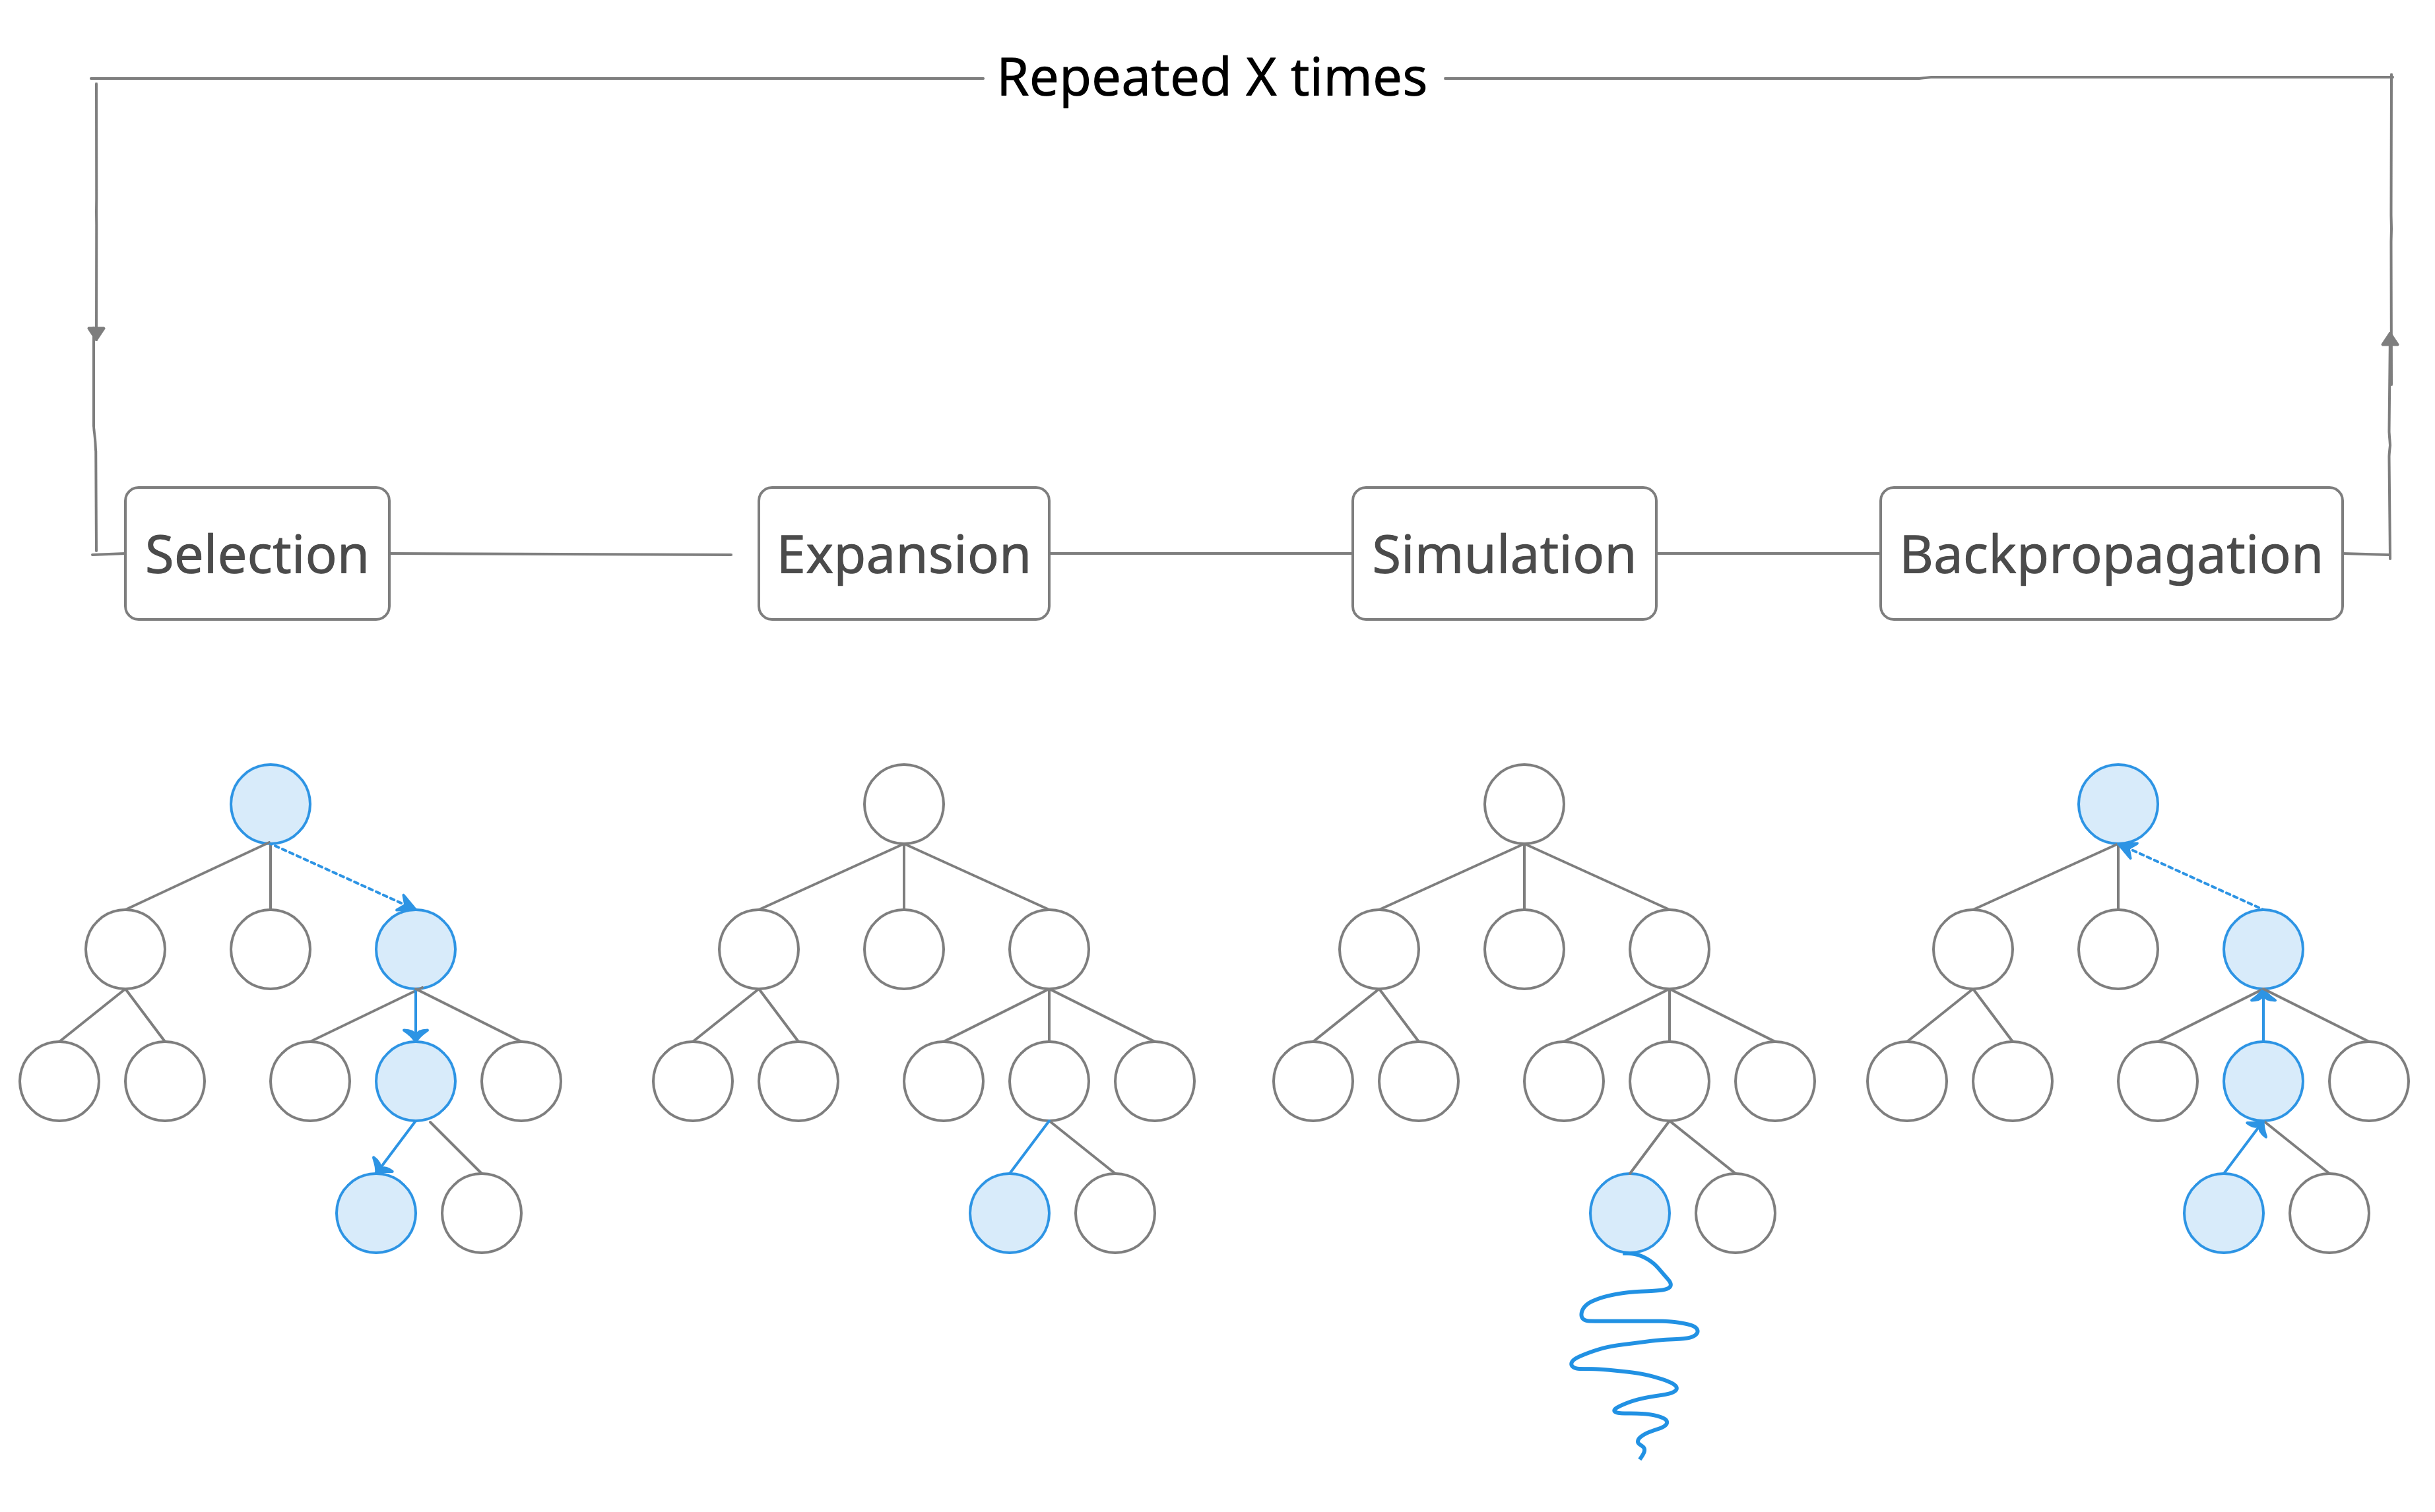
\includegraphics[width = \textwidth, height = 8cm]{Figures/MonteCarlo.png}
    \centering
\end{figure*}

\subsubsection{Aadapting Monte Carlo Tree Search to partially observable environments}
Despite the success of a sample-based approach, the extension of planning to uncertain (partially observable) environments still poses problems. 
In such an environemt (due to inperfect or incomplete observations), an agent is (initially) uncertain of the actual state. This causes considerable complexity, and has ramifications for the time and space requirements for computing an optimal policy. 
\newline \newline
In an $n$-stateful environment, an agent must compute a distribution over $n$ states representing its belief over the true state of the environment (also known as a belief-state). 
It must compute this in addition to the generic planning complexities of all possible actions, transitions and resulting states --- hence unless facing a very trivial problem in an exceedingly simple environment, the exponential complexity of partially observable environments tend to render planners inapplicable. 
\newline \newline
Silver and Veness  \cite{Silver2010} combined a sampling-based approach to belief updating (particle-filtering) with a monte-carlo tree search style algorithm which allows for partially observable planning. Among a number of alterations, each node in the tree is based on an observation history rather than a state, reflecting the agents belief over the state.  
\newline \newline
In small state spaces, the belief-state (i.e. distribution over the possible state) can be perfectly calculated by applying Bayes rule --- in large state spaces this can be computationally demanding, and a compact representation of the transition model (in terms of likelihoods) might not be available. To address this problem Silver and Veness contributed an algorithm, Partially Observable Monte Carlo Planning (POMCP), which uses a particle-filter: generating a number of small unweighted particles, each representing a possible state, and evaluating them based on expected vs received observations (as described in detail in Section \ref{ParticleFiter} and Section \ref{MCTSDesc}). They use this sampling-based approach to update the belief about the likely history at each time-step, and iteratively converge onto the true state.

\begin{figure*}
    \caption{Graphical representation of the POMCP architecture: the Simulator/Generative model is used both to reason over the apparent state based on an action history, but also to reason over the best possible action absed on a sample-based planner}
    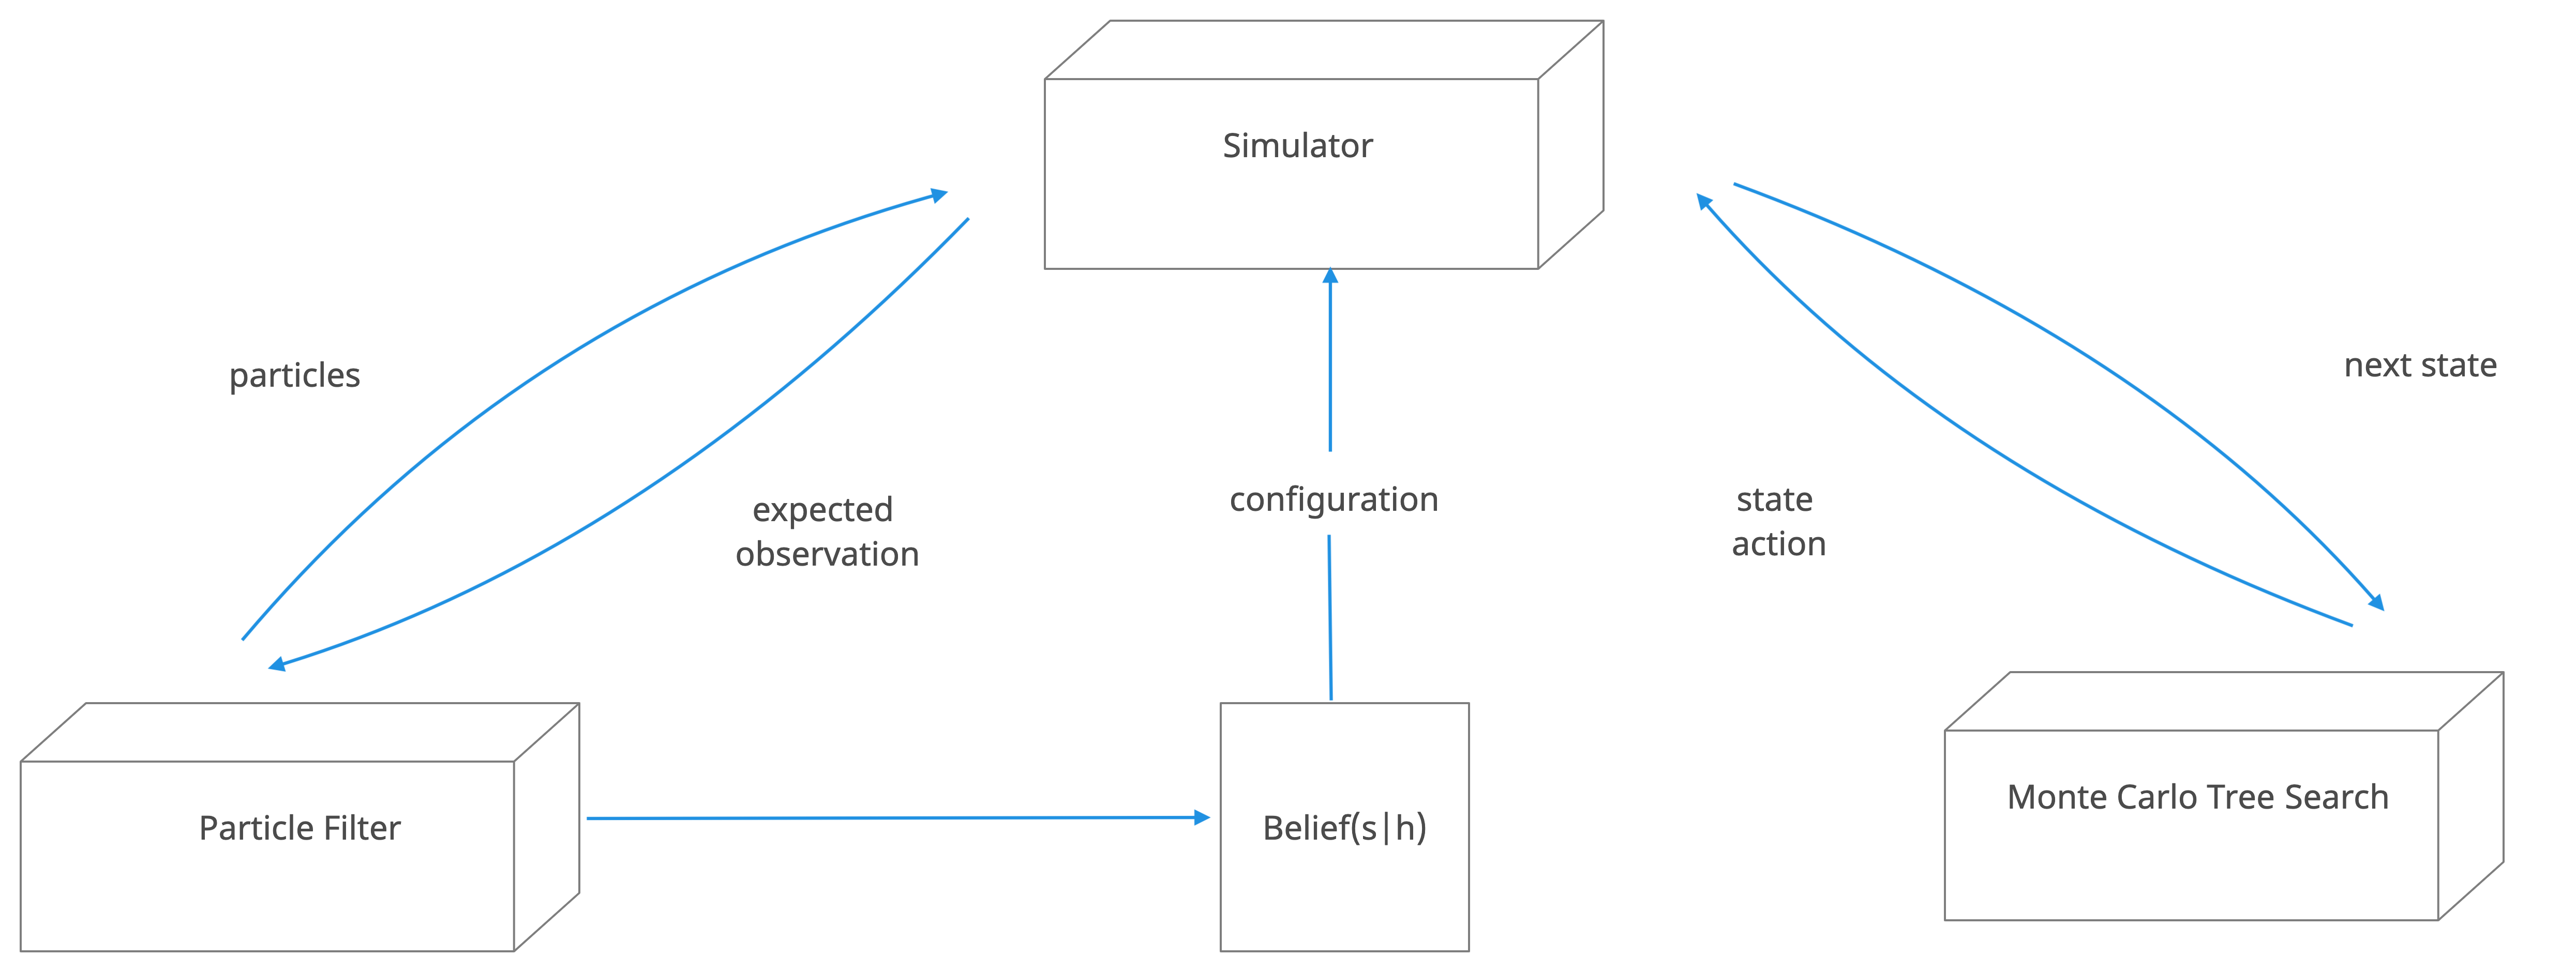
\includegraphics[width=\textwidth]{Figures/POMCP.png}
    \centering  
\end{figure*}

As with typical Monte Carlo methods, the sampling approach greatly limits the search space as only (likely) reachable states are evaluated, and the belief over states can be efficiently computed. In short, sampling based methods have shown to allow for swift approximation over complex belief spaces, and the combination of a particle filter with a Monte Carlo Tree Search allows for accurate estimation of the belief-state, and accurate approximation of a near-optimal policy despite complex environments.

\subsubsection{Improving on POMCP --- updating the environment simulation}  
Despite the theoretical success of POMCP, belief-based planning still poses challenges. 
While known for its efficacy in dealing with large state-spaces, MCTS is limited by the accuracy of the transition model. Simply put, if the model of the environment provided to the planner is not sufficiently expressive as to capture the environment dynamics, despite efficient sampling, the performance of an agent will be poor. 
\newline \newline
In recent years, there have been two notable works which have augmented belief-based planners with a learning capacity in order to overcome an incorrectly specified model. 
\newline \newline
Katt et al \cite{Katt2017} augmented the notation of a POMDP to take account of a number of extra features, to allow for a Bayesian updating of the environment model --- in effect the transition dynamics were updated as experience increased in a Bayesian way, allowing for more realistic rollouts and better action selection. In short, they incorportated a learning element into the model of the environment to allow for an incorrectly or incomplete black-box environment simulation. 
\newline \newline
With a similar aim, Hayashi et al \cite{Hayashi_et_al2020} augmented a POMCP planner with a deep-recurrent neural network as a mechanism for particle reinvigoration (suggesting possible states to evaluate), which suggested better candidate states (particles) to be computed allowing noisy or incorrectly specified environments to be used without resulting in poor agent performance. They phrased the environment simulator as a black-box with various parameters which required fitting. This fitting took place as experience grew, meaning that the black-box simulator could be tuned online, allowing the world-model to be iteratively updated. Crucially, they applied this to an opponent modelling task, the level-based foraging domain \cite{Papoudakis2020,Barrett2015}, in which agent types were parameters within the black-box simulator. 

\subsubsection{Incoporating agent models into MCTS}
As mentioned previously, a MCTS involves several stages: 1) traversing a tree via a best-first (heuristic) until reaching a leaf node; 2) Upon reaching a leaf node, it performs a rollout, which involves selecting an action, and sampling an environment simulator for a possible next state and expected reward. It continues this rollout to an arbitrary depth. 3) Finally, having reached a maximum depth, the reward is propagated back up the tree to the root node.
\newline \newline 
In a multi-agent environment, the transition function responsible for mapping one state to another depends on a \textit{joint action} taken by all agents. Hence, in a rollout, the simulator must assume a joint action (i.e. infer/suggest likely actions taken by \textit{other} agents). In this way, agent models are integrated into a MCTS via the simulation phase. In simple terms, they are implicitly included in the environment model --- this is defined mathematically in Section \ref{IncludingAgentModels}. In both \cite{Hayashi_et_al2020} and \cite{Albrecht_stone_2019} agent models are computed and viewed as parameters to be tuned in this environment, thus providing an interesting middle ground between a `global' approach, in which an agent simply learns a single generative model of  the environment from scratch (no opponent models), and a typical opponent modelling approach, which requires distinct agent models and environment models.
\newline \newline
This method also has benefits as it translates the problem of opponent modelling into one of state-space search.